% Instantaneous luminosity, $\mathcal{L} (t)$, is the rate at which colliding particles interact per unit area at a given moment in time. To determine the total number of interactions $N(t)$, the instantaneous luminosity is integrated over time and multiplied by the proton-proton interaction cross-section $\sigma_{pp}$, which characterizes the likelihood of a particular interaction:

% \begin{equation}
%     \centering
%     N(t) = \sigma_{pp} \int \mathcal{L} (t) dt
% \end{equation}

% \noindent{}The instantaneous luminosity can be defined as:

% \begin{equation}
%     \centering
%     \mathcal{L} = 2 N_1 N_2 f N_b \int \!\!\! \int \!\!\! \int \!\!\! \int_{-\infty}^{\infty} \rho_{1x}(x)\rho_{1y}(y)\rho_{1s}(s{-}s_0)\rho_{2x}(x)\rho_{2y}(y)\rho_{2s}(s{+}s_0)\, dx\, dy\, ds\, ds_0
% \end{equation}\label{eq:luminosity_long}

% \noindent{}where $N_1$ and $N_2$ are the number of particles per bunch, $f$ is the revolution frequency, $N_b$ is the number of bunches in one beam, and $\rho$ are the beam density distribution functions. Evaluating equation~\ref{eq:luminosity_long} is not always possible since all beam distributions need to be known. In many cases, it is appropriate to model these distributions as Gaussian.
% With this assumption, equation~\ref{eq:luminosity_long} simplifies to:

% \begin{equation}
%     \centering
%     \mathcal{L} = \frac{N_1 N_2 f N_b}{4\pi \sigma_x \sigma_y}
% \end{equation}

% \noindent{}The total integrated luminosity, $L$, is defined as the integral of the instantaneous luminosity over some time, $T$:
% \begin{equation}
%     \centering
%     L = \int_{0}^{T} \mathcal{L} (t) dt
% \end{equation}
% \noindent{}Thus it is seen that the total number of events is proportional to the total integrated luminosity.

% At the LHC, the nominal instantaneous luminosity is $\mathcal{L} = 10^{34} \mathrm{cm}^{-2}\mathrm{s}^{-1}$. During Runs 2 and 3, the recorded instantaneous luminosity approximately doubled the nominal value, reaching a sustained luminosity of $\mathcal{L} = 2.1 \cdot 10^{34} \mathrm{cm}^{-2}\mathrm{s}^{-1}$ for proton-proton collisions, while for heavy-ion collisions the maximum sustained luminosity recorded was $\mathcal{L} = 10^{27} \mathrm{cm}^{-2}\mathrm{s}^{-1}$~\cite{ATLAS_run3_luminosity_and_detector}. Figure~\ref{fig:atlas_luminosity_recorded} presents the total integrated luminosity delivered by the LHC and recorded by ATLAS during Run 3. Through the first three years of data taking for this run, the LHC has delivered a total of 195 $\mathrm{fb}^{-1}$ of data. Of this, ATLAS only recorded 183 $\mathrm{fb}^{-1}$ of data with only 169 $\mathrm{fb}^{-1}$ of data deemed suitable for physics analysis. These luminosity discrepancies
% arise when detector components malfunction or data-taking conditions change mid run. ATLAS maintains a record of periods with nominal conditions referred to as the ``Good Runs List'' (GRL), which defines the datasets available for further analysis.

% \begin{figure}
%     \centering
%     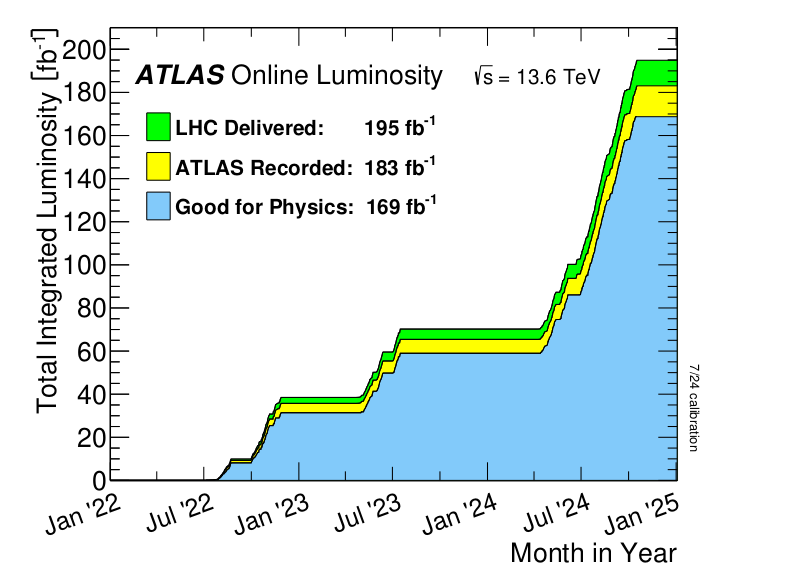
\includegraphics[width=0.8\textwidth]{figures/atlas/atlas_run3_lumi.png}
%     \caption{The total integrated luminosity delivered by the LHC and recorded by ATLAS\@. As seen in the figure, the LHC delivered and ATLAS recorded differ from one another due to non-nominal circumstances. Taken from~\cite{atlas_lumi_image}}\label{fig:atlas_luminosity_recorded}
% \end{figure}

%%% New revision
The instantaneous luminosity, $\mathcal{L}(t)$, is the rate of particle collisions per unit area at a given time. The total number of interactions, $N(t)$, is proportional to the integrated luminosity and the proton-proton- cross-section $\sigma_{pp}$
\begin{equation}
    \centering
    N(t) = \sigma_{pp} \int \mathcal{L} (t) dt
\end{equation}
The instantaneous luminosity is given by:
\begin{equation}
    \centering
    \mathcal{L} = 2 N_1 N_2 f N_b \int \!\!\! \int \!\!\! \int \!\!\! \int_{-\infty}^{\infty} \rho_{1x}(x)\rho_{1y}(y)\rho_{1s}(s{-}s_0)\rho_{2x}(x)\rho_{2y}(y)\rho_{2s}(s{+}s_0)\, dx\, dy\, ds\, ds_0
\end{equation}\label{eq:luminosity_long}
where $N_1$,$N_2$ are particles per bunch, $f$ the revolution frequency, $N_b$ number of bunches, and $\rho$ the beam density distribution functions. When the beam density distributions are modeled as Gaussians, this simplifies to
\begin{equation}
    \centering
    \mathcal{L} = \frac{N_1 N_2 f N_b}{4\pi \sigma_x \sigma_y}
\end{equation}
where $\sigma_x$ and $\sigma_y$ transverse beam widths. The integrated luminosity $L$ over time $T$ is defined as
\begin{equation}
    \centering
    L = \int_{0}^{T} \mathcal{L} (t) dt.
\end{equation}

At the LHC, the nominal instantaneous luminosity, $\mathcal{L} = 10^{34} \mathrm{cm}^{-2}\mathrm{s}^{-1}$, has been exceeded during Runs 2 and 3, and reached a sustained luminosity of $\mathcal{L} = 2.1 \cdot 10^{34} \mathrm{cm}^{-2}\mathrm{s}^{-1}$ in $pp$ collisions. For heavy-ions, peak instantaneous luminosity reached $\mathcal{L} = 10^{27} \mathrm{cm}^{-2}\mathrm{s}^{-1}$~\cite{ATLAS_run3_luminosity_and_detector}.

Figure~\ref{fig:atlas_luminosity_recorded} shows the integrated luminosity delivered to and recorded by ATLAS during Run 3\@. Of the 195 $\mathrm{fb}^{-1}$ delivered, 183 $\mathrm{fb}^{-1}$ were recorded and 169 $\mathrm{fb}^{-1}$ deemed suitable for physics analysis. The ``Good Runs List'' (GRL) defines the useable datasets and excludes periods with detector issues or unstable conditions.
\begin{figure}
    \centering
    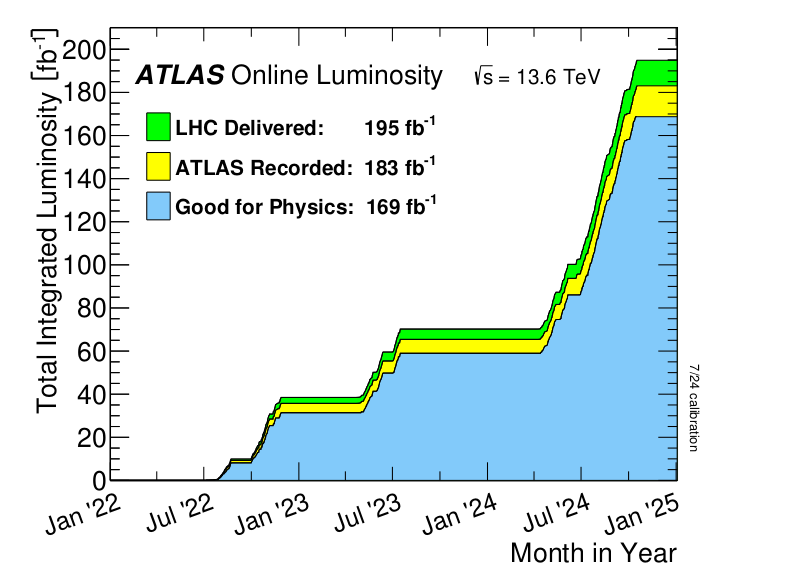
\includegraphics[width=0.8\textwidth]{figures/atlas/atlas_run3_lumi.png}
    \caption{Run 3 integrated luminosity delivered by the LHC and recorded by ATLAS\@. Differences reflect detector downtimes or suboptimal data-taking conditions. From~\cite{atlas_lumi_image}.}\label{fig:atlas_luminosity_recorded}
\end{figure}

High luminosity is required for observing the rare processes of interest at the LHC, but with it comes a key challenge: pileup. For every bunch crossing, there is one hard scattering process that produces the physics of interest, and many softer interactions that occur simultaneously and are called pileup. Pileup is quantified by the average number of interactions per bunch crossing, $\langle \mu \rangle$, which has increased throughout Run 3. In 2022 $\langle \mu \rangle = 43$, in 2023 $\langle \mu \rangle = 51$, and in 2024 $\langle \mu \rangle = 58$~\cite{atlas_pileup_image}. Mitigation strategies exist and include exploiting the granularity of the Inner Detector and various software-based techniques. Figure~\ref{fig:atlas_run3_pileup} shows the pileup distributions during the first three years of Run 3.

\begin{figure}
    \centering
    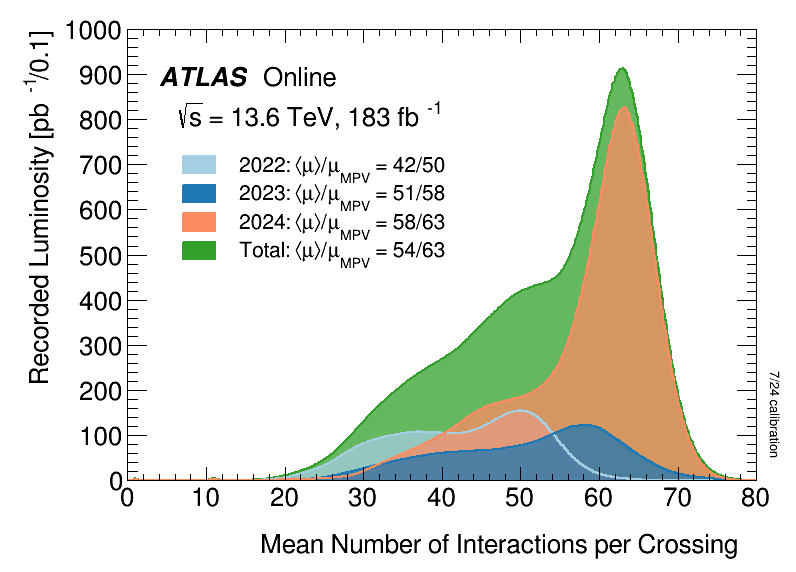
\includegraphics[width=0.8\textwidth]{figures/atlas/atlas_run3_pileup.png}
    \caption{The luminosity-weighted distribution for the mean number of interactions per bunch crossing for 2022--2024 pp collision data. Taken from~\cite{atlas_pileup_image}}\label{fig:atlas_run3_pileup}
\end{figure}